% Created 2022-11-08 Tue 11:11
% Intended LaTeX compiler: xelatex
\documentclass[11pt]{article}
\usepackage{graphicx}
\usepackage{grffile}
\usepackage{longtable}
\usepackage{wrapfig}
\usepackage{rotating}
\usepackage[normalem]{ulem}
\usepackage{amsmath}
\usepackage{textcomp}
\usepackage{amssymb}
\usepackage{capt-of}
\usepackage{hyperref}
\usepackage{geometry}[margin=0.25in]

\newcommand{\bigO}[1]{\mathcal{O}\left(#1\right)}

\author{Criston}
\date{\today}
\title{Hw\#1}

\graphicspath{{./figs/}}

\begin{document}

\maketitle

\textbf{Problem 1: Nondimensionalizing Navier Stokes}

Using the nondimensionalization given, show that eq 12-14 hold.

\textbf{Solution.}
Let
\begin{equation}
  \vec{u} =
  \begin{bmatrix}
    u\\ v\\ w
  \end{bmatrix}
\end{equation}
so that eqs (6)-(8) in the notes become the single vector valued equation:
\begin{equation}
  \label{eq:NS}
  \partial_t \vec{u} + \left(\vec{u}\cdot \nabla \right)\vec{u} = -\frac{1}{\rho}\nabla p + \nu \Delta \vec{u} + \frac{1}{\rho}\vec{f_b}
\end{equation}
I will omit the nondimensionalization of the incompressibility condition as it is trivial.

As in eqs (12-14) we neglect body forces $\vec{f_b} = \vec{0}$. Let $L,U,T$ be characteristic length, velocity, and time scales respectively, and note that $\rho = \text{constant}$ is the constant density of the incompressible fluid. Then we can define:
\begin{align}
  \label{eq:dimlessCoords}
  x',y',z' &= \frac{x}{L}, \frac{y}{L}, \frac{z}{L}\\
  \vec{u}' &= \frac{\vec{u}}{U}\\
  t' &= \frac{t}{T}\\
  p' &= \frac{p}{\rho U^2}
\end{align}
Then
\begin{align}
  \label{eq:dimlessOps}
  \partial_t &= \frac{1}{T}\partial_{t'}\\
  \nabla &= \frac{1}{L}\nabla'\\
  \Delta &= \frac{1}{L^2}\Delta'
\end{align}

Subsituting these definitions into eq(\ref{eq:NS}), we obtain
\begin{equation}
  \left( \frac{U}{T} \right) \partial_{t'} \vec{u}' + \left( \frac{U^2}{L} \right) \left(\vec{u}' \cdot \nabla'\right)\vec{u}'
  = \frac{\rho U^2}{\rho L} \nabla'p' + \frac{U}{L^2} \nu \Delta' \vec{u}'
\end{equation}
Finally, multiplying both sides by $\frac{L}{U^2}$ yields:
\begin{equation}
  \label{eq:nondimNS}
  \left( \frac{L}{TU} \right) \partial_{t'} \vec{u}' + \left(\vec{u}' \cdot \nabla'\right)\vec{u}'
  = \nabla'p' + \left( \frac{\nu}{LU} \right)\Delta' \vec{u}'
\end{equation}

And we define the two dimensionless numbers as in the text: $Re = \frac{LU}{\nu}$, $S = \frac{L}{TU}$. Note that if $T = L/U$, then $S = 1$.

\newpage

\textbf{Problem 2:} Convert the Navier-Stokes equations to cylindrical coordinates to show that stated equations hold.

\textbf{Solution.}
We begin with the incompressibility condition and Navier-Stokes (for notational simplicity I will drop the vector symbol and allow context to differentiate scalar and vector):
\begin{equation}
  \label{eq:incom}
  \nabla \cdot u = 0
\end{equation}
\begin{equation}
  \label{eq:NS_2}
  \partial_t u + (u \cdot \nabla)u = -\frac{1}{\rho}\nabla p + \nu \Delta u
\end{equation}

We use the simplifying assumptions that the flow is steady ($\partial_tu=0$), rotationless ($\partial_\theta = 0$, $u_\theta = 0$), so that eq(\ref{eq:NS_2}) becomes
\begin{equation}
  \label{eq:simpleNS}
  (u \cdot \nabla)u = -\frac{1}{\rho}\nabla p + \nu \Delta u
\end{equation}

I now write the $\nabla$ and $\Delta$ operators in cylindrical coordinates, using the simplifications above. Let $f$ be a scalar-valued function and $A$ be a vector-valued function, and let a vector in cylindrical coordinates be written in component form as $A = (A_r, A_\theta, A_x)$ where $r$ is the radial direction, $\theta$ the rotation, and $x$ the lengthwise direction.
\begin{align}
  \label{eq:nablaCyl}
  \nabla f &= \left( \partial_r f, 0, \partial_x f \right)\\
  \nabla \cdot A &= \frac{1}{r} \partial_r(rA_r) + \partial_x A_x\\
  \nabla^2 f &= \frac{1}{r} \partial_r \left( r \partial_r f \right) + \partial_{xx}f\\
  \nabla^2 A &= \left( \frac{1}{r} \partial_r (r \partial_r A_r) + \partial_{xx}A_r - \frac{A_r}{r^2}, 0, \frac{1}{r}\partial_r(r\partial_r A_x) + \partial_{xx}A_x\right)
\end{align}

Incompressibility equation becomes
\begin{equation}
  \nabla \cdot u = 0 \implies \frac{1}{r} \partial_r(ru_r) + \partial_x(u_x) = 0
\end{equation}
And Navier-Stokes becomes, (component by component)
\begin{align}
  r \text{ component}:&\\
                      &u_r \partial_r u_r + u_x \partial_xu_r = -\frac{1}{\rho}\partial_rp + \nu \left(\frac{1}{r}\partial_r(r\partial_r u_r) + \partial_{xx}u_r - \frac{u_r}{r^2}\right)\\
  \theta \text{ component}:&\\
                      &0\\
  x \text{ component}:&\\
                      &u_r\partial_ru_x + u_x\partial_xu_x = -\frac{1}{\rho}\partial_xp + \nu \left(\frac{1}{r}\partial_r(r\partial_ru_x)+\partial_{xx}u_x\right)
\end{align}
\newpage

\begin{figure}
  \centering
  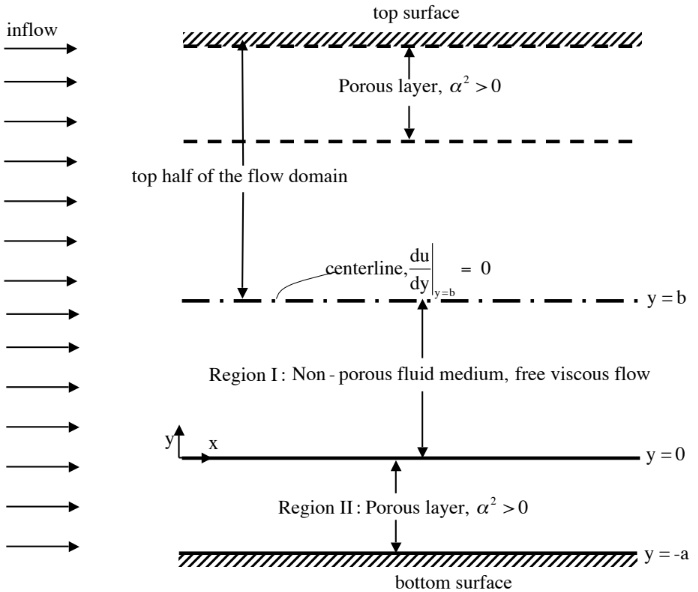
\includegraphics[width=0.5\textwidth]{prob3.png}
  \caption{Problem 3 setup}
  \label{fig:prob3}
\end{figure}

\textbf{Problem 3: Channel flow between porous layers}

Derive a simplified two-dimensional representation of flow between porous layers. Consider a channel as shown in figure \ref{fig:prob3}. The flow field is assumed symmetric about the centerline $y=b$, and the analysis should be restricted to the bottom half of the system. The flow is assumed to be steady $(u_t = 0)$ and fully developed $u_x = 0$, and zero in cross-stream direction $(v=0)$.

\textit{Region I:} Write the simplified $x$-momentum equation within the free shear flow region $\alpha^2 = 0$ along with appropriate boundary condtions.

\textit{Region II:} Write down appropriate boundary conditions and simplified equations of motion.

Solve coupled system of ODEs.


\textbf{Solution.}
Beginning from the 2D Brinkman equations:
\begin{align}
  \partial_t u + u\partial_xu + v\partial_yu &= -\frac{1}{\rho}\partial_xp+\nu\left(\partial_{xx}u + \partial_{yy}u\right) + \alpha^2 \mu u\\
  \partial_t v + u\partial_xv + v\partial_yv &= -\frac{1}{\rho}\partial_yp+\nu\left(\partial_{xx}v + \partial_{yy}v\right) + \alpha^2 \mu v
\end{align}

We apply the simplifications: zero in cross-stream ($v = 0$), steady ($\partial_tu = 0$), fully developed ($\partial_xu=0$), to obtain the simplified momentum equations:
\begin{align}
  0 &= -\frac{1}{\rho}\partial_xp + \nu \partial_{yy}u + \alpha^2\mu u \label{eq:pmom}\\
  0 &= -\frac{1}{\rho}\partial_yp
\end{align}
From the above we have $p(x,y) = p(x)$.

\textbf{In region I}, $\alpha = 0$ so that eq(\ref{eq:pmom}) becomes
\begin{equation}
  0 = -\frac{1}{\rho}\partial_xp + \nu \partial_{yy}u\label{eq:reg1}
\end{equation}
with boundary conditions
\begin{align}
  \partial_yu(y=b) &= 0 \label{eq:bc1.1}\\
  \lim_{y\to 0^+}u &= \lim_{y\to 0^-}u \label{eq:bc1.2}
\end{align}

Then, solving eq(\ref{eq:reg1}) by direct integration:
\begin{equation}
  u(y) = \left(\frac{y^2}{2\nu \rho}\right)\partial_xp + Ay + B
\end{equation}
Applying BC eq(\ref{eq:bc1.1}):
\begin{equation}
  \partial_yu(y=b) = 0 \implies -\left(\frac{b}{\nu \rho}\right)\partial_xp = A 
\end{equation}

So that
\begin{equation}
  \label{eq:insolreg1}
  u(y) = \left( \frac{\partial_x p}{\nu \rho} \right)\left( \frac{1}{2}y^2 - by + C\right)
\end{equation}
where $C$ is some yet-to-be-determined constant. Finally, note that
\begin{equation}
  \label{eq:leftlim}
  \lim_{y\to 0^+}u(y) = \left( \frac{\partial_x p}{\nu \rho} \right)C
\end{equation}

\textbf{Turning to region II}, eq(\ref{eq:pmom}) becomes (denoting $u\to u^*$ to help differentiate)
\begin{equation}
  0 = -\frac{1}{\rho}\partial_xp + \nu \partial_{yy}u^* + \alpha^2\mu u^* \label{eq:reg2}
\end{equation}
with boundary conditions
\begin{align}
  u^*(y=-a) &= 0 \label{eq:bc2.1}\\
  \lim_{y\to 0^+}u &= \lim_{y\to 0^-}u^* \label{eq:bc2.2}
\end{align}

To solve eq(\ref{eq:reg2}), one would normally add the general solution to the homogenous equation to a particular solution for the inhomogenous equation. However, the general solution to the homogenous equation is simply the trivial zero function, so we only need to find a particular solution. I take the anzatz $u^*(y) = Ay^2+By+D$. Differentiating we find that
\begin{equation}
  u^*(y) = \left( -\frac{\partial_xp}{\rho \alpha^2 \mu} \right)y + D
\end{equation}
After applying eq(\ref{eq:bc2.1}), and enforcing eq(\ref{eq:bc1.2}):
\begin{equation}
  \boxed{
    \begin{aligned}
      u(y) &= \left( \frac{\partial_xp}{\nu \rho} \right) \left(\frac{1}{2}y^2 -by - \frac{a\nu}{\alpha^2\mu}\right)\\
      u^*(y) &= \left(-\frac{\partial_xp}{\rho \alpha^2 \mu}\right)(y+a)
    \end{aligned}
  }
\end{equation}

\end{document}